% Created 2012-10-03 Wed 00:07
\documentclass[11pt]{article}
\usepackage[utf8]{inputenc}
\usepackage[T1]{fontenc}
\usepackage{fixltx2e}
\usepackage{graphicx}
\usepackage{longtable}
\usepackage{float}
\usepackage{wrapfig}
\usepackage{soul}
\usepackage{textcomp}
\usepackage{marvosym}
\usepackage{wasysym}
\usepackage{latexsym}
\usepackage{amssymb}
\usepackage{hyperref}
\tolerance=1000
\usepackage{setspace} \onehalfspace
\providecommand{\alert}[1]{\textbf{#1}}

\title{Pony Design Document}
\author{Andrew K. Hirsch}
\date{\today}

\begin{document}

\maketitle


\section{Introduction}
\label{sec-1}


Imagine you are a soldier in, say, the American Revolution. You have just been granted a rifle, and you want to customize it to fit your particular style. You have two options: you can add a longer barrel, or you can add a bayonet. The longer barrel allows you to take more accurate shots, and the bayonet allows you to fight at a short distance.

This sort of customization of tools is common in many fields. Programmers even have it to some degree; many heavily customize the environment that they code in. But what every programmer deals with on a daily basis is the language that they code in, which is, in many cases, completely non-customizable. Pony wants to give this sort of power to a programmer in their language, so that programmers can use the tools that they are most comfortable with.

However, if you add a bayonet to your gun with a longer barrel, then the longer barrel will keep the bayonet from doing what you want. This is an important point with customization: two customizations may interfere with each other. In this case, it is impossible to use both of them at the same time. To do so would be logically impossible. This does not change when we are talking about programming languages rather than weapons.

Pony attempts to detect when a programmer is attempting to use such customizations. This is actually impossible in the general case; however, we attempt to do so for as many cases as possible. This is a significant theoretical contribution, and is not at all trivial.

Pony is written in Haskell, which allows us to prove properties. Haskell forces us to write in a purely functional style. In order to allow for these customizations, we must write a program that can take a customized language as input. However, nobody has written such a program in a purely functional style before, at least not that is published in the literature. Writing such a program is also a technical challenge and contribution of Pony.
\section{Core Requirements}
\label{sec-2}


\begin{itemize}
\item Allow users to use programming language constructs in C.
\begin{itemize}
\item Allow users to use Objects, including class-based and prototype-based.
\item Allow users to use Lists, such as one might find in LISP or Haskell.
\end{itemize}
\item Allow users to use these constructs in embedded systems.
\begin{itemize}
\item By compiling to ANSI C, this comes naturally.
\end{itemize}
\item Allow users to develop new programming languages, and compile them to C.
\begin{itemize}
\item By allowing users arbitrary control of syntax and semantic transformation, it is possible to use Pony to write a compiler for i.e. Javascript.
\end{itemize}
\end{itemize}
\section{List of Functions}
\label{sec-3}

Because Pony is in its second development phase, there are three pieces of functionality to focus on:

\begin{itemize}
\item Collision detection for semantic transformations
\begin{itemize}
\item When a transformation's action may work on the action of another transformation, the user should be alerted to this possibility.
\item When a transformation's action \underline{will} work on the action of another transformation on a particular piece of code, Pony should recognize this as an error.
\end{itemize}
\item Languages for writing extensions and semantic transformations
\begin{itemize}
\item Pony will have to parse these languages, so that it can feed them to interpreters or translators.
\item Pony will have to interpret these languages, using them in its processes, or translate them into a language it can use.
\end{itemize}
\item A parsing function (Written using Parsec)
\begin{itemize}
\item We need to be able to parse arbitrary formal languages, so that Pony can work with extended languages that do not follow C syntax rules.
\item We need to write a function for extending a pre-written parser, so that transformations can be written without specifying the entire language.
\end{itemize}
\end{itemize}
\section{Use Cases}
\label{sec-4}


\begin{itemize}
\item A user wants to write C code with a new construct.
\begin{itemize}
\item If the construct has already been written as a transformation, then the user can simply use that transformation.
\item Otherwise, the user must define a transformation before writing with it.
\end{itemize}
\item A user wants to write a new language and Compile to C
\begin{itemize}
\item The parser should no longer accept C code at this point.
\item The user must specify the syntax of the language as well as how it is transformed into C code.
\end{itemize}
\item A user wants to write a new extension and publish it for others.
\begin{itemize}
\item Some extensions (i.e. Objects) may be standard.
\item This means that transformations must be generalized and publishable!
\end{itemize}
\end{itemize}
\section{Data Structures}
\label{sec-5}

Since Pony is written in Haskell, we eschew C-style data structures for the most part, preferring type-theoretic data structures such as sum types and records. However, we will also be making extensive use of linked lists, a FP standard, and trees, a compiler standard. Pony will also use monads and other category-theoretic data structures. Most of these are baked in either to Haskell or the pre-existing Pony code.
\section{Key Algorithms}
\label{sec-6}

The main algorithm that is going to be introduced will be unification, which will be used for collision detection. Also important will be monad composition and transformation, combinator libraries, and \underline{Data Types a la Carte}-style extensibility. The GHC API or its derivatives might come into play, but will hopefully not.



\begin{figure}[htb]
\centering
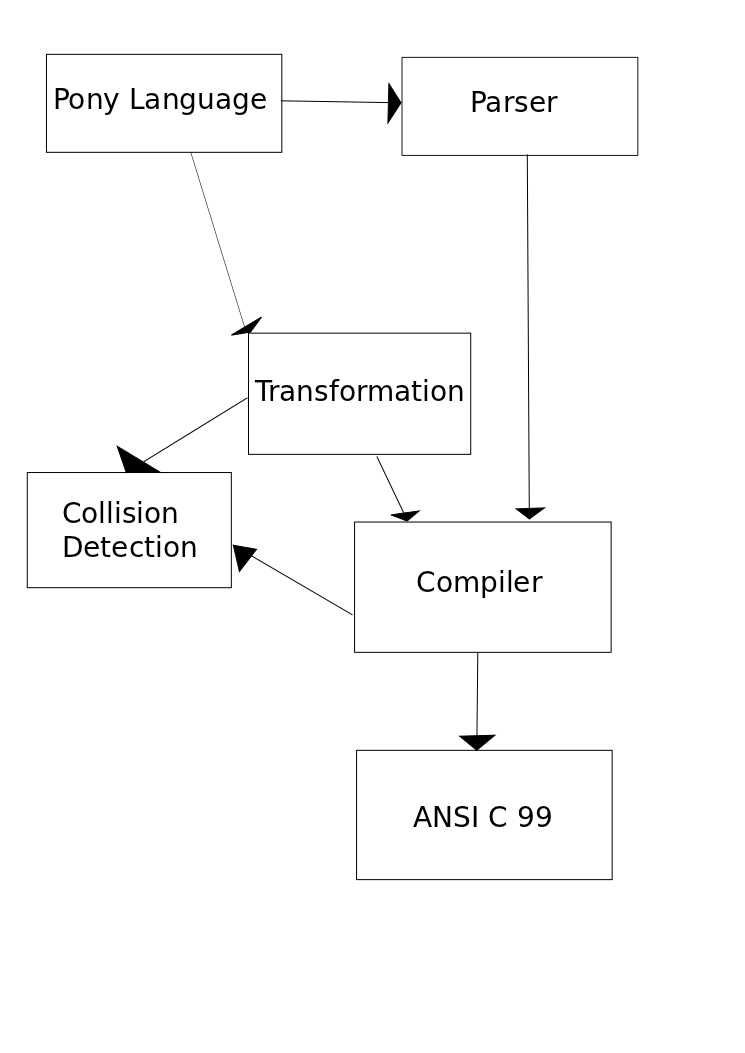
\includegraphics[width=10cm]{./components.png}
\caption{\label{fig:modules}Pony Modules}
\end{figure}

\end{document}
